\section{You have to see the \ch{O2}!}\label{sec:see_the_O2}

Materials with high oxygen evolution activity are often reported in the literature. A common benchmark is the overpotential required to reach 10 mA/cm$^2$\cite{McCrory2013, Kibsgaard2019}. This value is usually normalized to the macroscopic, i.e. \textit{geometric}, electrode area, rather than the electrochemical surface area, which is not trivial to determine for oxides. For this reason, many advances in activity are in fact just advances in synthesizing electrodes with a very high loading\cite{Kibsgaard2019}. There is nothing wrong with this in principle - a high geometric loading of active sites enables electrochemical devices such as electrolyzer cells to be more compact, lowering capital costs - though it should be thought of as an engineering accomplishment, to be kept conceptually separate from more fundamental catalysis science, which seeks to increase the activity per active site\cite{Seh2017}. There is, however, the problem with high-loading materials that the large amount of material means that charging or degradation phenomena can involve the passage of a lot of charge. This can lead to an overestimation of the activity if 100\% Faradaic efficiency to the OER (Reaction \ref{rxn:OER4}) is assumed blindly. Especially bad is if the material contains organic building blocks, as all organic molecules are unstable with respect to oxidation to \ch{CO2} at OER potentials. Thus, just as an example, there is reason to be skeptical of the reported activity of the high-surface-area metal-organic-framework (MOF) derived \ch{Cr_{0.6}Ru_{0.4}O_x} catalyst described by Lin et al in ref. \citen{Lin2019}, which currently claims a record\cite{Kibsgaard2019} of 178 mV overpotential at 10 mA/cm$^2$. Charging, degradation, and oxidation of residual carbon could all contribute to the current of these electrodes, even over a long experiment. Measurement of dissolved metals using ICP-MS or mass losses using quartz crystal microbalance can check for degradation processes\cite{Frydendal2014}. But the best way to prove that the measured current is going to OER is to quantitatively measure the evolved \ch{O2}. 

Here, I report two examples from my PhD work of OER catalysts, the first in acid and the second in alkaline, for which the measured current was not all going to \ch{O2} production via Reaction \ref{rxn:OER4}.

\subsection{Ru on graphene oxide}

\begin{figure}[b!]
	\centering
	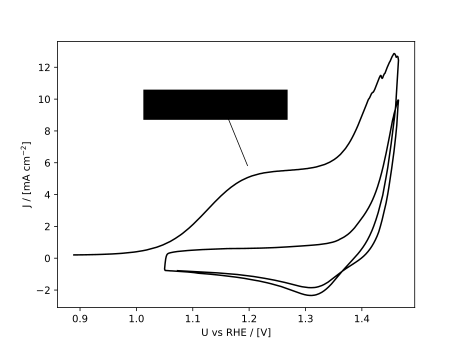
\includegraphics[width=0.5\textwidth]{04_Oxygen/fig/Ru_on_GO_naive.png}
	\caption{Initial cyclic voltammagrams of Ru on graphene oxide material from the lab in Fuzhou, in 0.5 M \ch{H2SO4}}
	\label{fig:Ru_on_GO_naive}
\end{figure}

During my external stay with professor Wen Zhenhai in Fuzhou, one of the first measurements we did with their newly built EC-MS setup (Appendix \ref{app:Fuzhou}) was to determine the actual onset of OER from an acid electrocatalyst that they knew was unstable (the overpotential required to draw 10 mA started low but skyrocketed after a few minutes), but appeared highly active. This material, dispersed ruthenium on a high-surface-area graphene oxide, showed a strong oxidation wave starting before 1.4 V vs RHE with a large shoulder starting at 1.2 V vs RHE (Figure \ref{fig:Ru_on_GO_naive}). It was of interest whether all of the current in the wave at 1.4 V, or even 1.2 V if the catalyst was somehow ultra-activated in the beginning, could be attributed to \ch{O2} formation.

\begin{figure}[t]
	\centering
	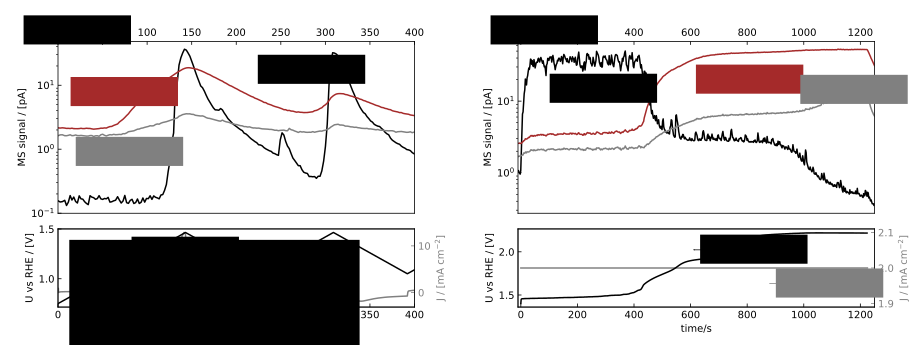
\includegraphics[width=1\textwidth]{04_Oxygen/fig/Ru_on_GO.png}
	\caption{EC-MS plots of Ru on graphene oxide material from the lab in Fuzhou, in 0.5 M \ch{H2SO4}. \textbf{(a)} initial cyclic voltammagrams and \textbf{(b)} constant-current experiment.}
	\label{fig:Ru_on_GO}
\end{figure}

Figure \ref{fig:Ru_on_GO}a shows the same cyclic voltammatry data with mass spectrometry detection of the products. Clearly, the ``ultra-low onset \ch{O2}'' above is not \ch{O2} but instead is revealed by the m/z=44 signal, implying \ch{CO2} evolution, to be oxidation of the graphene oxide support. This oxidation of the support continues into the main OER wave, and can also be seen in the second cycle. The onset for \ch{O2}, at about 1.33 V vs RHE, is remarkably low, indicating that the catalyst is highly active (though perhaps only as active as \ch{RuO2} films, see Section \ref{sec:low_O2}). However, there is less \ch{O2} in the second cycle, belying the catalyst's instability.

Figure \ref{fig:Ru_on_GO}b shows a 20-minute constant-current measurement in the EC-MS setup. At 2 mA/cm$^2$, it fails catastrophically at around 400 seconds into the experiment. At this point, the potential increases rapidly, and the 2 mA/cm$^2$ no longer goes to OER, but instead goes to oxidation of the substrate, as indicated by the switch from m/z=32 (\ch{O2}) to m/z=44 (\ch{CO2}) in the mass spectrometer. This is likely the point at which all of the ruthenium has dissolved or detached from the substrate. There is a m/z=28 signal which is attributed to fragmentation of \ch{CO2}, but, interestingly, at about 1100 s, the m/z=28 signal starts increasing independently of the m/z=44 signal. This is attributed to a new mechanism for oxidation of the carbon support at these high potentials ($>$2 V vs RHE) resulting in evolution of \ch{CO}. 

This illustrates the importance of product detection when measuring activity in the highly corrosive acid OER conditions.

\subsection{Nickel-iron: electrodeposited film vs annealed nanoparticles}\label{subsec:NiFe}

\begin{figure}[b!]
	\centering
	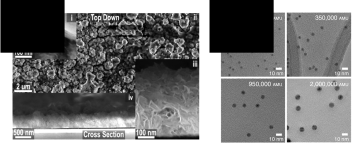
\includegraphics[width=1\textwidth]{04_Oxygen/fig/NiFe_foam_and_NPs.png}
	\caption{SEM images of NiFe-based OER catalysts \textbf{(a)}, Example of a high-loading, high-surface-area NiFe oxyhydroxide catalyst studied in the literature, taken from reference \citen{Batchellor2015}. \textbf{(b)}, Mass-selected vacuum-synthesized NiFe nanoparticles, from Paper \ref{Roy2018}.}
	\label{fig:NiFe_foam_and_NPs}
\end{figure}

As mentioned above, electrodes based on oxidized nickel and iron are used in industrial alkaline electrolyzer cells. However, the intrinsic OER activity of this electrocatalytic material is not well known, since it is typically used and studied in a highly porous foamy form\cite{Dionigi2016b}. An example, from ref \citen{Batchellor2015}, is shown in Figure \ref{fig:NiFe_foam_and_NPs}a. It is very difficult to estimate the intrinsic activity, i.e., the turn-over-frequency, of such materials because it is hard to determine how many active sites are accessible for the reaction. This was our primary motivation for studying a model system: vacuum-synthesized mass-selected \ch{Ni_{0.75}Fe_{0.25}} nanoparticles, characterized in detail in Paper \ref{Roy2018}.

The mass-selected nanoparticles were formed in a cluster source as follows\cite{VonIssendorff1999}: 
\begin{enumerate} 
	\item Atoms were freed from a solid metallic target (here \ch{Ni_{0.75}Fe_{0.25}}) by bombardment with a magnetically-bound plasma, i.e. magnetron sputtering. 
	
	\item These atoms were condensed into nanoparticles with a wide size distribution in an aggregation zone with a controlled temperature and argon pressure. Many of the nanoparticles are ionized, i.e. they carry a fundamental charge. 
	
	\item The charged nanoparticles are accelerated into a separation chamber and filtered according to m/z ratio using a modified time-of-flight mass spectrometer. 
	
	\item The beam of mass-selected nanoparticles is directed to a conductive substrate (here a 5mm Au stub) which is grounded via an ampmeter.  \label{item:deposition}
\end{enumerate}

The deposition current, measured in part \ref{item:deposition} above of the deposition technique, tells the number of nanoparticles deposited, since each deposited nanoparticle carries a fundamental charge. Since the size of the particles is known, this means that the mass loading is also known. Making an assumption about the shape of the nanoparticles, this means that the surface area is also known. In the case of the NiFe nanoparticles described here, SEM images (Figure \ref{fig:NiFe_foam_and_NPs}b) confirm a spherical shape. This is especially useful, because it means, assuming the electrochemical reaction only occurs on the surface of the catalyst, that the number of available atomic sites can be calculated, and the turn-over frequency thus determined. These assumptions and results are discussed in more detail in Paper \ref{Roy2018} and in Section \ref{sec:lattice_O}.


\begin{figure}[t]
	\centering
	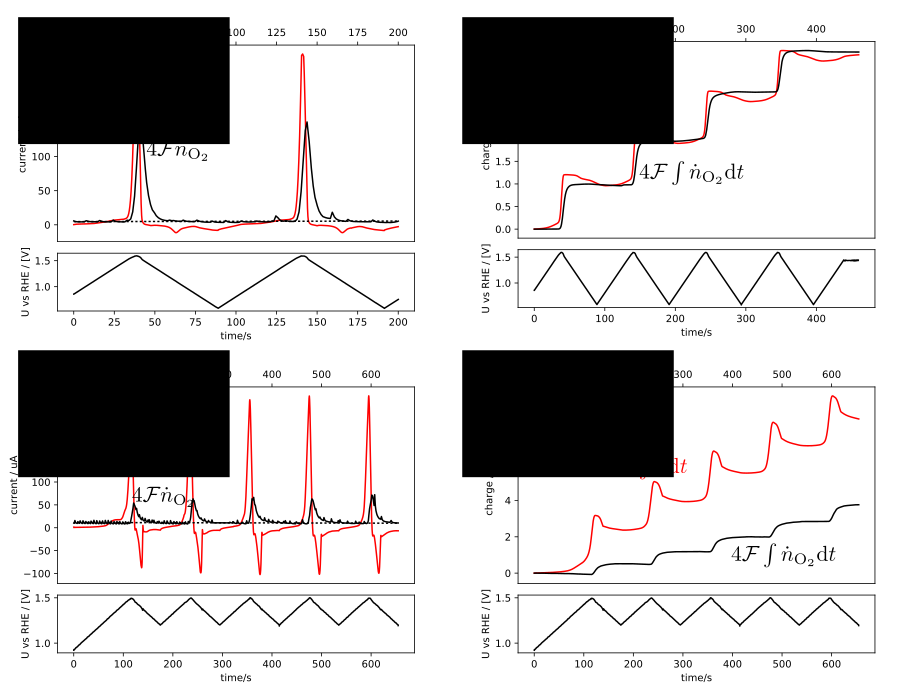
\includegraphics[width=1\textwidth]{04_Oxygen/fig/NiFe_current_vs_O2.png}
	\caption{Comparison of the electrode current and the OER current equivalent of the \ch{O2} signal in 0.1 M KOH for \textbf{(a-b)} 7 nm thermally annealed \ch{Ni_{0.75}Fe_{0.25}O_x} nanoparticles and \textbf{(c-d)} an electrodeposited \ch{Ni_{0.75}Fe_{0.25}O_xH_y} film. \textbf{(a)} and \textbf{(c)} show the (partial) current densities, while \textbf{(b)} and \textbf{(d)} show the integrals thereof.}
	\label{fig:NiFe_current_vs_O2}
\end{figure}

SEM and TEM images of the mass-selected nanoparticles also confirm that they are unchanged before and after reaction (Figures 2 and 4 of Paper \ref{Roy2018}). The OER activity is also stable over 1000 hours at 1.6 V vs RHE. These observations, taken together with the very small loading of the samples (approximately 150 ng of total Ni and Fe), indicate that charging or dissolution processes are negligible. We confirmed this using EC-MS by comparing the measured electrode current and the \ch{O2} signal during cyclic voltammatry in 0.1 M KOH of a sample with 150 ng of 7 nm mass-selected \ch{Ni_{0.75}Fe_{0.25}O_x} nanoparticles (the metal nanoparticles were annealed in \ch{O2} in the vacuum chamber for this sample). The results are shown in Figure \ref{fig:NiFe_current_vs_O2}a. The \ch{O2} signal, calibrated to mol/s as described in Chapter \ref{ch:Tools}, is multiplied by four times Faraday's constant $\mathcal{F}$, which is the charge passed per mol of \ch{O2} formed by water oxidation, in order to plot on the same axis as the electrode current. The integrated current and the integrated OER partial current, shown in Figure \ref{fig:NiFe_current_vs_O2}b, match. This makes it clear that all of the net current can be accounted for by OER. The oscillating contribution of the \ch{Ni^{2+}/Ni^{3+}} cancels itself out when integrated.

For comparison, we synthesized a porous \ch{Ni_{0.75}Fe_{0.25}} oxy-hydrodixe film by electrodeposition, according to the method described in ref. \citen{Trotochaud2014a}, typical for the synthesis of \ch{NiFe}-based films studied in the literature\cite{Dionigi2016b}. In short, a current of $-0.2$ mA/cm$^2$ was passed through the substrate (a 5 mm Au stub) for 5 min in an electrolyte containing 100 mM \ch{Ni(NO3)2 * 6 H2O} and 5 mM \ch{FeCl2}. We then perform the same EC-MS experiment comparing the electrode current and evolved \ch{O2} during the first cyclic voltammagrams (Figure \ref{fig:NiFe_current_vs_O2}c and d). Unlike the case for the thermally oxidized nanoparticles, they do not match up over time. There is some net current transfer which cannot be accounted for by water oxidation. This may be attributed to charging of the film or dissolution of the metals, particularly Fe, which is known to leach. It could also be due to oxidation of adsorbed carbon-containing species (advantitious carbon), which would not be observed in EC-MS since the evolved \ch{CO2} would be captured by the alkaline electrolyte as \ch{CO3^{2-}}.

These results further highlight the need to measure \ch{O2} when determining the OER activity, especially for high-loading catalysts. Electrodeposited NiFe oxy-hydroxide films are known to be stable over longer periods of time, and are closely related to the catalyst used industrially in alkaline electrolyzer cells, but Figure \ref{fig:NiFe_current_vs_O2} makes it clear that, if \ch{O2} is not measured, one could easily overestimate the activity by just looking at the current passed during cyclic voltammatry.